\documentclass[12pt]{article}
\usepackage[a4paper, total={6in, 8in}]{geometry}
\usepackage[utf8]{inputenc}
\usepackage{booktabs}
\usepackage{rotating}
\usepackage{multirow}
\usepackage[graphicx]{realboxes}
\usepackage{stackengine}
\usepackage{epigraph}
\usepackage{float}
\usepackage{dcolumn}
% \usepackage{longtable}
\usepackage{supertabular}
% \usepackage[nomarkers]{endfloat}
\usepackage{acronym}
\usepackage{listings}
\usepackage{hyperref}
\hypersetup{colorlinks=true,%
citecolor=black,%
filecolor=black,%
linkcolor=black,%
urlcolor=black
}
\usepackage[portuguese]{babel}
\usepackage[autostyle,portuguese=brazilian]{csquotes}
\usepackage{setspace} % for \onehalfspacing and \singlespacing macros
\onehalfspacing
\usepackage{etoolbox}
\usepackage{amsmath}
\AtBeginEnvironment{quote}{\singlespacing\small}
% \usepackage[usestackEOL]{stackengine}
\usepackage[justification=centering]{caption}
\usepackage[notes,backend=biber]{biblatex-chicago}
\usepackage{subfig} %incluir Figura side by side
%codigo  para spacing 1.5
%\usepackage{setspace}
%\doublespacing
%codigo para monospace justificado tt
\renewcommand{\familydefault}{\rmdefault}
%codigo estilo dos numeros
\usepackage[sc,osf]{mathpazo}
\usepackage{ragged2e}
\justifying

\usepackage{listings}
\usepackage{xcolor}

\definecolor{codegreen}{rgb}{0,0.6,0}
\definecolor{codegray}{rgb}{0.5,0.5,0.5}
\definecolor{codepurple}{rgb}{0.58,0,0.82}
\definecolor{backcolour}{rgb}{0.95,0.95,0.92}

\lstdefinestyle{mystyle}{
    backgroundcolor=\color{backcolour},   
    commentstyle=\color{codegreen},
    keywordstyle=\color{magenta},
    numberstyle=\tiny\color{codegray},
    stringstyle=\color{codepurple},
    basicstyle=\ttfamily\footnotesize,
    breakatwhitespace=false,         
    breaklines=true,                 
    captionpos=b,                    
    keepspaces=true,                 
    numbers=left,                    
    numbersep=5pt,                  
    showspaces=false,                
    showstringspaces=false,
    showtabs=false,                  
    tabsize=2
}

\lstset{style=mystyle}

\bibliography{references.bib}

\usepackage{enumitem}
\newlist{floatnotes}{description}{1}
\setlist[floatnotes]{font=\normalfont\itshape,wide, nosep, leftmargin=.1\linewidth, itemindent=\labelsep, rightmargin=\leftmargin, before=\vspace{.5em}\footnotesize}

\usepackage{pdflscape}
\usepackage{afterpage}
\usepackage{capt-of}% or use the larger `caption` package
\usepackage{enumitem}

\makeatletter
%Add packages here
\usepackage{hyperref}

\begin{document} 

\newgeometry{margin = 1.05in, top=1.05in}
\linespread{1.1}

\title{%
  O Índice ESG de Equidade Racial: conceito, visão setorial e aspectos práticos da adesão
}
\author{Pacto de Promoção da Equidade Racial \thanks{Responsáveis técnicos: Lucas Cavalcanti Rodrigues e Crislane Alves Bastos}}

\maketitle

\section*{Introdução}
\addcontentsline{toc}{section}{Introdução}

\par Esse relatório trata do Índice ESG de Equidade Racial (IEER), proposto pelo Pacto de Promoção da Equidade Racial --- organização sem fins lucrativos dedicada à promoção da diversidade no ambiente corporativo brasileiro. O documento é dirigido principalmente às empresas parceiras do Pacto e tem como principal objetivo detalhar o IEER, metodológica e empiricamente, e mostrar como empresas aderentes do Pacto podem usar a métrica para ajudar a melhorar a diversidade do seu quadro de colaboradores, bem como contribuir para tornar o Brasil um país mais justo e igualitário.

\par O presente documento está dividido em mais 3 seções. Na seção seguinte, apresenta-se uma descrição dos três níveis do IEER, como definido no documento de lançamento do Pacto.\footnote{O documento está disponível online no site do Pacto (\hyperlink{http://pactopelaequidaderacial.org.br/assets/files/PACTO-DEPROMOODAEQUIDADERACIAL-PaperInstrutivo-1.12.2021-1.pdf}{link})}. Em seguida, na seção \ref{sectors}, apresenta-se os resultados do cômputo do nível 1 do IEER para cada setor da economia. Essa análise setorial considera todos os subsetores da economia definidos pelo IBGE, mas particular atenção é dada ao setor bancário. Na seção \ref{als_study} realiza-se uma simulação do IEER para uma empresa fictícia. No exemplo, mostra-se os resultados da empresa, compara-se com seu respectivo setor e detalha-se como mudanças nos níveis 2 e 3 do IEER podem afetar o indicador de equidade racial global da empresa.

\clearpage

\section{O Índice ESG de Equidade Racial} \label{ieer_levels}

\par O Índice ESG de Equidade Racial (IEER) é composto por três níveis. No primeiro nível, doravante $IEER^{I}$, o índice é uma métrica que procura diagnosticar o \textit{status} atual de equidade racial da empresa, comparando a proporção de negros entre os colaboradores da empresa com a proporção de negros na localidade em que a empresa atua.\footnote{Usando a terminologia da Relação Anual de Informações Sociais, são chamados negros neste documento os trabalhadores classificados como pretos ou pardos.} O segundo nível, chamado $IEER^{II}$, é o indicador de equidade racial da empresa após serem consideradas a adoção de ações afirmativas, que contemplem o recrutamento, permanência e promoção de profissionais negros. Por fim, o terceiro nível $IEER^{III}$ é o indicador de equidade racial da empresa que, além de considerar a adoção de ações afirmativas, também considera os investimentos sociais voltados à equidade racial.\footnote{Conforme relata o documento de lançamento do pacto, os investimentos considerados no nível 3 devem dar preferência a organizações com lideranças negras já atuantes e fomentar a criação de novas organizações negras}

\par É importante notar que, embora composto, o \textit{IEER} da empresa é um indicador único que considera o resultado do $IEER^{I}$ somado aos pontos obtidos pela empresa nos $IEER^{II}$ e $IEER^{III}$. Na subseção seguinte, detalha-se o cômputo do $IEER^{I}$, que serve de base para os demais indicadores. Esta seção é bem técnica e pode ser pulada por leitores interessados em aspectos mais gerais do indicador. Nas subseções \ref{levels2} e \ref{levels3}, mostra-se como funciona o sistema de pontos nos níveis  $IEER^{II}$ e $IEER^{III}$.

\subsection{Nível I: definição e detalhes técnicos} \label{level1}

\par Para o cômputo do \textit{IEER}, computa-se, primeiramente um índice chamado $Index_{rs}$ para as ocupações da empresa ou setor. O $Index_{rs}$ é um índice que mede o grau de desigualdade racial em uma ocupação específica e têm esse nome em referência aos autores que primeiro propuseram sua fórmula de cálculo.\autocite{ransom2001one} Depois de computado, o $Index_{rs}$ é agregado a nível da empresa ou setor usando o vetor da massa salarial das ocupações como ponderador. A seguir, detalha-se o procedimento de cálculo.

\par Assume-se que a probabilidade de $x$ trabalhadores negros estarem ocupados em uma ocupação $j$, com $n$ trabalhadores segue uma distribuição binomial:

\begin{equation}
P_{j}(X=x_{j})=\binom{n_{j}}{x_{j}}p^{x_{j}}(1-p)^{n_{j}-x_{j}}
\end{equation}

\par Usando propriedades da distribuição binomial, é possível definir o nível de equilíbrio racial de uma determinada ocupação pela diferença da quantidade de negros observados na ocupação ($x_{j}$) e seu valor esperado ($n_{j}p$). Medindo essa distância no número de desvios-padrões temos:

\begin{equation}
\label{eqv}
v_{j} = \frac{x_{j} - n_{j}p}{\sqrt{n_{j}p(1-p)}}
\end{equation}

\par  O $Index_{rs}$ é apenas uma versão padronizada do índice anterior (detalhes algébricos da padronização do índice encontram-se no anexo \ref{standard_ieer}). Valores próximos a -1 representam baixa proporção relativa de negros na ocupação \textit{j}. No outro extremo, um $Index_{rs}=1$ significa que negros são sobre-representados na ocupação \textit{j}.

\par Definido dessa forma, o $Index_{rs}$ já é utilizado na literatura econômica.\autocite{ransom2001one, rodriguescinzas} Para chegar no IEER usado pelo pacto, realiza-se uma agregação do índice ocupacional a nível da empresa ou setor (subscrito \textit{i}), usando a massa salarial (\textit{W}) como vetor de ponderação:
\begin{equation}
    IEER_{i}(\textbf{b}|p) = \sum_{j=1}^{J}\left[\left(\frac{b_{i,j}-p}{p}\right)\left(\frac{p}{1-p}\right)^{b_{i,j}}\right] \cdot \frac{W_{i,j}}{W_{i}}
    \label{eq_2}
\end{equation}

\par A agregação apresentada anteriormente é feita para três grupos de ocupação: diretoria, gerência e demais ocupações (chamadas não-liderança). Por fim, uma empresa têm um indicador global chamado IEER Ponderado que é a média aritmética dos três indicadores anteriores. Assim, para cada empresa existem 4 indicadores: IEER Diretoria, IEER Gerência, IEER não-liderança e IEER Ponderado.

\subsection{Nível II: Ações Afirmativas} \label{levels2}

\par Após comprometer-se com metas de incremento do seu $IEER^{I}$, recomenda-se à empresa a
adoção de ações afirmativas com potencial de melhorar o $IEER^{I}$ no curto, médio e longo prazo. Para cada ação afirmativa adotada (dentre as abaixo elencadas), serão somados +0,04 pontos ao $IEER^{II}$ da empresa, ficando limitado a +0,20 pontos ou a 1/3 do déficit do $IEER^{I}$ (o que for menor).

\par São as ações afirmativas sugeridas:
\begin{itemize}
    \item Política de recursos humanos e de contratação com foco no aumento da equidade racial (ex.:
    processos seletivos exclusivos ou com cotas para negros), priorizando a contratação,
    retenção e promoção de profissionais negros qualificados já disponíveis na própria empresa
    ou no mercado (até 0,04 pontos)
    \item Adoção de critérios e políticas de equidade racial para a seleção/exclusão de parceiros
    (fornecedores, distribuidores, prestadores de serviços, terceiro setor e comunidade) (até
    0,04 pontos)
    \item Adoção de práticas administrativas e projetos de mudança cultural para a valorização da
    diversidade e eliminação de fontes de discriminação direta e indireta, com a realização de
    ações para o letramento racial das lideranças e de recenseamento racial interno com base
    em auto declaração pelos colaboradores, seguindo parâmetros definidos pelo Conselho do
    Pacto e/ou indicação por Certificadora (até 0,04 pontos)
    \item Estabelecimento de objetivos e indicadores e métricas que possibilitem o monitoramento do
    impacto e da eficácia das políticas de valorização da diversidade (até 0,04 pontos)
    \item Criação de canais de denúncias de situações de assédio moral e de discriminação de caráter
    racial, de gênero, de pessoas com deficiência e de orientação afetivo-sexual (até 0,04
    pontos)
\end{itemize}


% EQUATION

\par Assim, caso uma empresa adote 3 das ações afirmativas sugeridas, ela terá um incremento de até +0,12
(ou seja, 3 x +0,04) em seu $IEER^{II}$, sendo este número limitado a 1/3 do gap entre o $IEER^{I}$ da
empresa e zero (o que indica uma empresa com equilíbrio racial)


\subsection{Nível III: Investimento Social em Equidade Racial} \label{levels3}

\par O ganho de pontos no indicador $IEER^{III}$ estará limitado a +0,20 pontos ou a 1/3 do déficit do
$IEER^{I}$ (o que for menor) e é condicional ao estabelecimento de metas para a melhoria do $IEER^{I}$ e à adoção de ações afirmativas (vide $IEER^{II}$).

\par O ganho dependerá do investimento social voltado à equidade racial com foco em educação e
mercado de trabalho. Assim, caso a empresa realize 100\% do investimento social calculado com
base no valor de referência ela contará com um incremento de +0,20 em seu $IEER^{III}$ e caso realize,
por exemplo, 40\% do investimento esperado o ganho será proporcional, de +0,08 pontos.

\par O Investimento Social de Referência (ISR) é calculado com base no custo de formação anual de
jovens negros suficientes para que a empresa alcance o equilíbrio racial ($IEER^{I}$ = 0), estando
limitado a R\$ 30 milhões/ano por grupo econômico. Assim, para uma empresa com \textit{m} ocupações, onde a proporção de negros em uma ocupação \textit{j} é novamente representada por $b_{j}$ e \textit{p} é a proporção de negros na população de referência, o ISR será dado por:

\begin{equation}
    ISR = \sum_{j=1}^{m} (p-b_{j}^{em})\cdot n_{j}^{em}\cdot 6.000 + \sum_{j=1}^{m} (p-b_{j}^{es})\cdot n_{j}^{es}\cdot 12.000
\end{equation}

\par Onde os sobrescritos \textit{em} e \textit{es} referem-se a ensino médio e ensino superior, respectivamente. A fórmula considera a estimativa de custos médios com a formação educacional de qualidade no
Brasil para:

\begin{itemize}
    \item Ensino Fundamental/Médio: custo anual aproximado de R\$ 6,0 mil/aluno com base em estudo do Todos pela Educação que – com dados de 2015 – estima em R\$ 4,3 mil o Valor Anual por Aluno (VAA) da educação básica pública a partir do qual não existem evidências de ganhos marginais em notas do IDEB. O VAA aproximado de R\$ 6,0 mil é alcançado ao se atualizar o valor de R\$ 4,3 mil pelo INPC acumulado até 2021, ficando próximo também do VAA efetivo de importantes redes de ensino básico como Ceará, Espírito Santo, Goiás e São Paulo (vide dados do SIOPE-FNDE para 2018 e 2019).

    \item Ensino Superior: custo anual aproximado de R\$ 12,0 mil/aluno com base na mensalidade de
    faculdades privadas e filantrópicas brasileiras ranqueadas no THE – Times Higher Education 2021.
\end{itemize}

\section{Análise setorial} \label{sectors}

\par Nesta seção, apresenta-se os resultados da implementação do $IEER^{I}$ para os setores e grupos de atividade econômica no Brasil. A tabela 1 apresenta um sumário da estimação do $IEER^{I}$ para 25 subsetores da economia, enquanto a tabela 2 detalha os resultados para cada subsetor individualmente. É possível identificar ao menos dois padrões pela observação da tabela. Em primeiro lugar, é notável que a maior parte dos subsetores da economia são caracterizados por forte sub-representação de negros. Este resultado é esperado, já que negros são sabidamente sobre-representados entre desempregados e trabalhadores do setor informal e os dados da RAIS, usados nesse relatório, cobrem apenas o setor formal da economia.

% Isso porque o setor com melhor indicador de equidade racial (Construção Civil) apresenta uma moderada sub-representação de negros, com $IEER^{I}$ de -0.20.

% \begin{table}[htb!] 
% \centering
% \caption{Sumário do Índice ESG de Equidade Racial - 25 subsetores - Estado de São Paulo - 2020}
% \begin{tabular}{lcccc} 
% \hline
%               & Não-Liderança & Gerência & Diretoria & Ponderado \\ \hline
% Média         & -0.26         & -0.59    & -0.76    & -0.54     \\
% Desvio-Padrão & 0.17          & 0.13     & 0.12     & 0.12      \\
% Mínimo        & -0.63         & -0.75    & -0.93    & -0.72     \\
% 25\%          & -0.31         & -0.69    & -0.82    & -0.61     \\
% 50\%          & -0.26         & -0.60    & -0.79    & -0.55     \\
% 75\%          & -0.18         & -0.52    & -0.70    & -0.50     \\
% Máximo        & 0.16          & -0.28    & -0.47    & -0.24     \\ \hline
% \end{tabular}
% \begin{floatnotes}
% \item [Fonte:] RAIS 2020.
% \end{floatnotes}
% \end{table}


\begin{table}[htb!]
\centering
\caption{Sumário do Índice ESG de Equidade Racial - 25 subsetores - Brasil - 2020}
\resizebox{\textwidth}{!}{%
\begin{tabular}{lcccc}
\toprule
\multicolumn{1}{c}{\textbf{}} & Não-Liderança & Gerência & Diretoria & Ponderado \\ \midrule
Média & -0.44 & -0.53 & -0.68 & -0.55 \\
Desvio-Padrão & 0.08 & 0.10 & 0.12 & 0.09 \\
Mínimo & -0.60 & -0.74 & -0.90 & -0.72 \\
25\% & -0.51 & -0.63 & -0.78 & -0.60 \\
50\% & -0.47 & -0.54 & -0.69 & -0.57 \\
75\% & -0.37 & -0.45 & -0.59 & -0.49 \\
Máximo & -0.20 & -0.35 & -0.43 & -0.37 \\ \bottomrule
\end{tabular}%
}
\begin{floatnotes}
\item [Fonte:] RAIS 2020.
\end{floatnotes}
\end{table} \label{tab_summary_sector}

\par Um segundo fato que pode ser observado na tabela é que, em geral, os indicadores de equidade racial em posições de não-liderança são melhores dos o que se observa em posições gerência que, por sua vez, são melhores que os indicadores para posições de diretoria. Como pode ser observado na tabela \ref{tab:all_sectors} que detalha o resultado do $IEER^{I}$ para cada subsetor, a tendência da desigualdade racial piorar conforme se sobe na hierarquia ocupacional é bastante difundida em todos os setores.


\clearpage

\afterpage{%
    \clearpage% Flush earlier floats (otherwise order might not be correct)
    \thispagestyle{empty}% empty page style (?)
    \begin{landscape}% Landscape page \
        \captionof{table}{Índice ESG de Equidade Racial - 25 subsetores - Brasil - 2020}% Add 'table' caption
        \centering % Center table
            % Please add the following required packages to your document preamble:
% \usepackage{graphicx}
\begin{table}[htb!]
\centering
\resizebox{\textwidth}{!}{%
\begin{tabular}{lccccc}
\hline
Sub-Setor IBGE                                                      & Não-Liderança & Gerência & Diretoria & Ponderado & Total Trabalhadores \\ \hline
Comércio varejista                                                  & -0.35         & -0.41    & -0.59     & -0.45     & 9,170,718.00        \\
Com. e administraçao de imóveis, valores mobiliários, serv. Técnico & -0.37         & -0.51    & -0.6      & -0.5      & 7,764,745.00        \\
Serv. de alojamento, alimentaçao, reparaçao, manutençao, redaçao    & -0.36         & -0.44    & -0.68     & -0.49     & 5,250,064.00        \\
Transportes e comunicaçoes                                          & -0.34         & -0.51    & -0.58     & -0.48     & 3,160,438.00        \\
Construçao civil                                                    & -0.2          & -0.43    & -0.52     & -0.38     & 2,987,343.00        \\
Indústria de produtos alimentícios, bebidas e álcool etílico        & -0.39         & -0.45    & -0.69     & -0.51     & 2,828,138.00        \\
Serviços médicos, odontológicos e veterinários                      & -0.43         & -0.42    & -0.54     & -0.46     & 2,641,732.00        \\
Agricultura, silvicultura, criaçao de animais, extrativismo vegetal & -0.34         & -0.35    & -0.43     & -0.37     & 2,074,241.00        \\
Comércio atacadista                                                 & -0.45         & -0.54    & -0.71     & -0.57     & 1,996,199.00        \\
Ensino                                                              & -0.48         & -0.46    & -0.56     & -0.5      & 1,796,329.00        \\
Instituiçoes de crédito, seguros e capitalizaçao                    & -0.51         & -0.59    & -0.69     & -0.6      & 1,378,833.00        \\
Ind. química de produtos farmacêuticos, veterinários, perfumaria    & -0.49         & -0.64    & -0.79     & -0.64     & 1,151,194.00        \\
Administraçao pública direta e autárquica                           & -0.49         & -0.4     & -0.46     & -0.45     & 1,002,717.00        \\
Indústria têxtil do vestuário e artefatos de tecidos                & -0.49         & -0.56    & -0.72     & -0.59     & 969,383.00          \\
Indústria metalúrgica                                               & -0.44         & -0.57    & -0.69     & -0.57     & 782,709.00          \\
Indústria mecânica                                                  & -0.53         & -0.74    & -0.8      & -0.69     & 656,492.00          \\
Indústria do material de transporte                                 & -0.59         & -0.65    & -0.89     & -0.71     & 532,427.00          \\
Indústria da madeira e do mobiliário                                & -0.52         & -0.57    & -0.81     & -0.63     & 485,348.00          \\
Serviços industriais de utilidade pública                           & -0.47         & -0.51    & -0.77     & -0.59     & 477,193.00          \\
Indústria de produtos minerais nao metálicos                        & -0.44         & -0.63    & -0.69     & -0.59     & 428,137.00          \\
Ind. da borracha, fumo, couros, peles, similares, ind. diversas     & -0.51         & -0.67    & -0.78     & -0.65     & 417,338.00          \\
Indústria do papel, papelao, editorial e gráfica                    & -0.51         & -0.56    & -0.7      & -0.59     & 366,372.00          \\
Indústria de calçados                                               & -0.6          & -0.66    & -0.9      & -0.72     & 337,618.00          \\
Indústria do material elétrico e de comunicaçoes                    & -0.48         & -0.63    & -0.7      & -0.6      & 325,044.00          \\
Extrativa mineral                                                   & -0.36         & -0.5     & -0.78     & -0.54     & 242,496.00          \\ \hline
\end{tabular}%
}
\begin{floatnotes}
\item [Fonte:] RAIS 2020.
\end{floatnotes}
\end{table} \label{tab:all_sectors}
    \end{landscape}
    \clearpage% Flush page
}

\clearpage
\subsubsection{Histórico do setores}
\par Aqui, apresenta-se os resultados da evolução do IEER para setores selecionados, a saber: i) Comércio varejista; ii) Comércio e administração de imóveis, valores mobiliários, serviços técnico; iii) Serviços de alojamento, alimentaçao, reparaçao, manutençao, redaçao; e, iv)  Transportes e comunicações. O critério de seleção para estes foi o maior número de empregabilidade.

    \begin{figure}[htb!]
        \centering
        \caption{Evolução do IEER - Setores da Economia}
            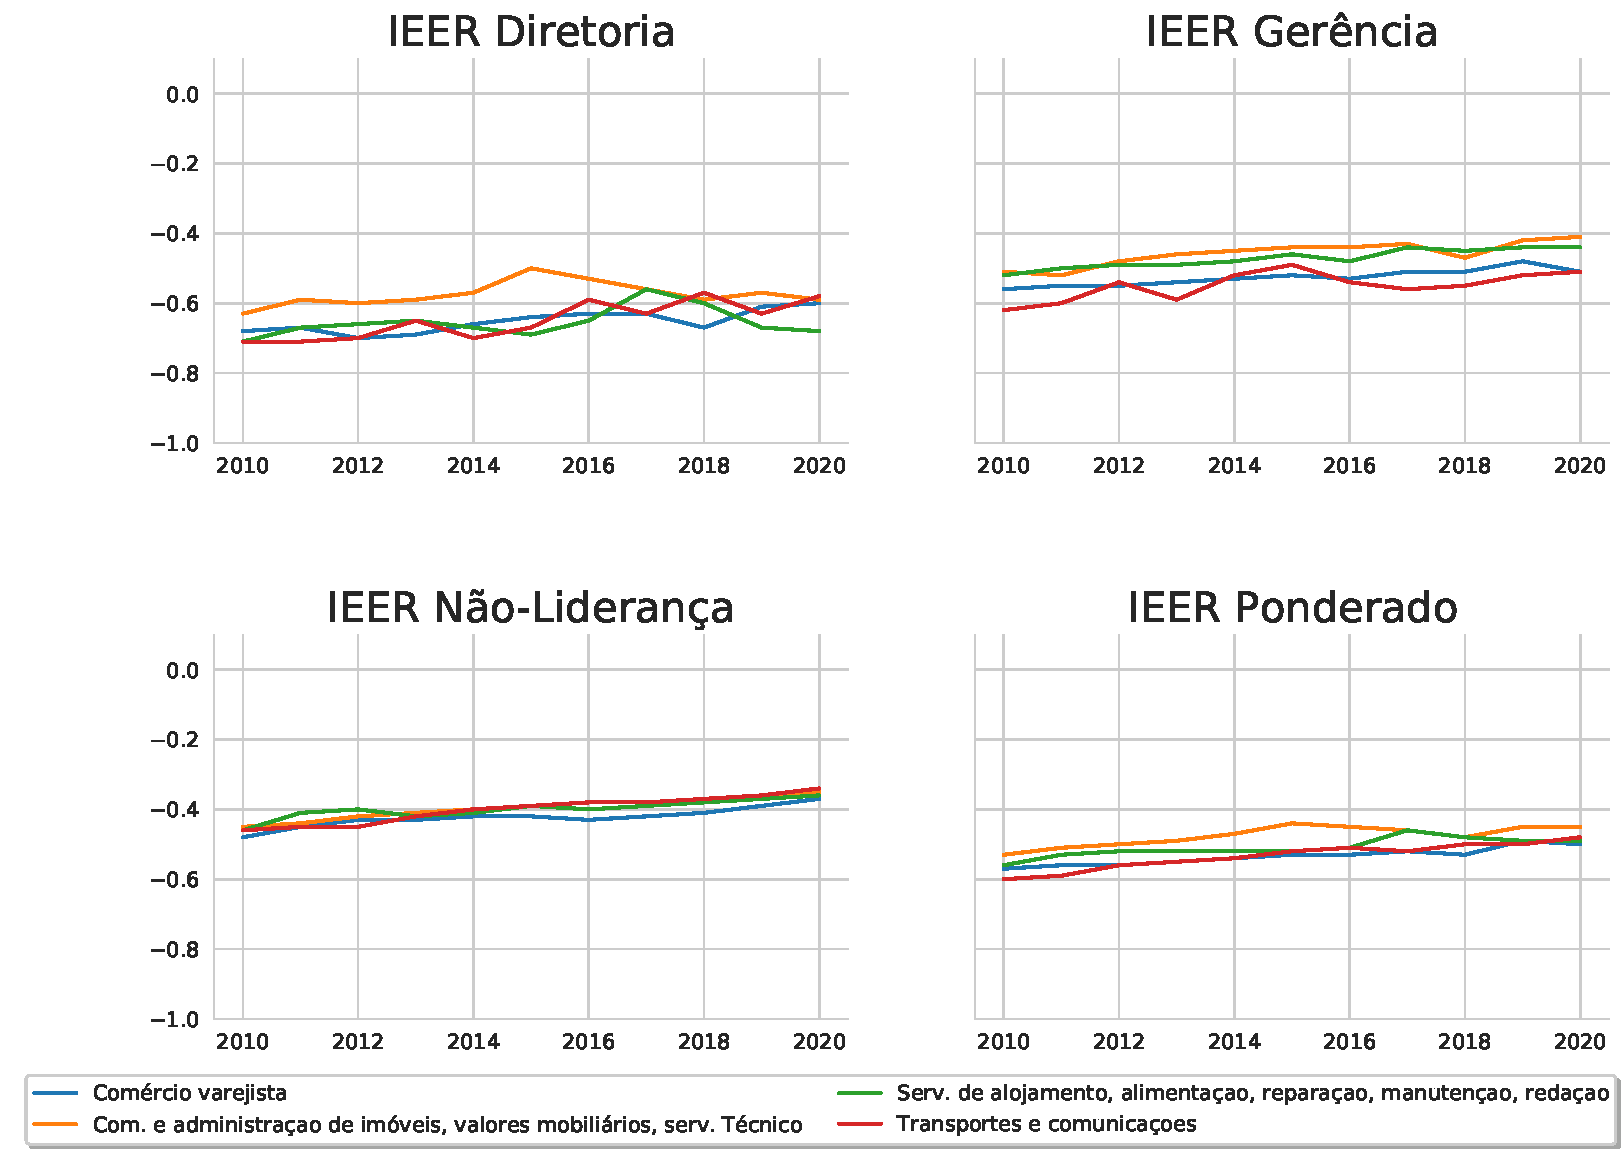
\includegraphics[height=12cm]{images/ieer_brasil_setor_2010_2020.pdf}
        \label{fig1}
    \end{figure} \label{setor_ts}

\par Todos os setores apresentam aumentos no ponderado ao longo dos anos. O maior deles é o de Transporte e Comunicações, que apresentava um ponderado (-0,60) em 2010 e (-0,48) em 2020. O segundo melhor resultado é o setor de Comércio e administração de imóveis com ponderado de -0,53 e -0,45 em 2010 e 2020, respectivamente. O setor Varejista (-0,57 e -0,50) e o de Serviços de alojamento (-0,56 e -0,49), não se diferenciam muito apresentando resultados mais modestos do que os anteriores. 

\par Os dados apresentados nas tabelas 1 e \ref{tab:all_sectors} e na figura 1, ilustram muito bem como o $IEER^{I}$ se comporta em diferentes setores da economia. Fica clara que o grau de desigualdade racial é elevado na maioria dos setores da economia e é especialmente pronunciado quando se analisa ocupações de liderança. No entanto, o grau de agregação da classificação de subsetores do IBGE é muito elevado e acaba por incluir no mesmo grupo empresas com elevada heterogeneidade de porte, receita, composição de capital humano, entre outros fatores. Como forma de contornar essa limitação, apresenta-se a seguir uma análise focada em subgrupos de empresas no setor bancário. A análise utilizou 5 grupos da CNAE, seguindo nomenclatura usada pela FEBRABAN. Assim, os grupos avaliados a seguir e suas respectivas CNAEs são Bancos Comerciais (64.21-2), Bancos de Investimentos (64.32-8), Bancos Múltiplos com Carteira Comercial (64.22-1), Bancos Múltiplos sem Carteira Comercial (64.31-0) e Caixas Econômicas (64.23-9).

\subsection{Desigualdade racial no setor bancário}

\par Nesta subseção, foca-se em grupos selecionados de atividade econômica dentro do setor de \enquote{Instituições de crédito, seguros e capitalização}. Foram selecionados cinco grupos de empresas, quais sejam, bancos comerciais e de investimento, caixas econômicas e bancos múltiplos, com e sem carteira. Os resultados para cada um destes setores, para os anos de 2010 e 2020, são apresentados a seguir.

\begin{table}[htb!]
\centering
\caption{Índice ESG de Equidade Racial - Bancos Comerciais - Brasil - 2010/2020}
\begin{tabular}{lcccc}
\hline
Ano  & Não-Liderança & Gerência & Diretoria & Ponderado \\ \hline
2010 & -0.87          & -0.84    & -0.96     & -0.89     \\
2011 & -0.74          & -0.74    & -0.93     & -0.8      \\
2012 & -0.79          & -0.85    & -0.97     & -0.87     \\
2013 & -0.72          & -0.78    & -0.95     & -0.82     \\
2014 & -0.82          & -0.9     & -0.91     & -0.88     \\
2015 & -0.79          & -0.88    & -0.94     & -0.87     \\
2016 & -0.8           & -0.78    & -0.96     & -0.85     \\
2017 & -0.77          & -0.83    & -0.96     & -0.86     \\
2018 & -0.79          & -0.85    & -0.97     & -0.87     \\
2019 & -0.75          & -0.88    & -0.96     & -0.86     \\
2020 & -0.75          & -0.86    & -0.93     & -0.85     \\ \hline
\end{tabular}
\begin{floatnotes}
\item [Fonte:] RAIS 2010-2020.
\end{floatnotes}
\end{table}

\begin{table}[htb!]
\centering
\caption{Índice ESG de Equidade Racial - Bancos de Investimento - Brasil - 2010/2020}
\begin{tabular}{lcccc}
\hline
Ano  & Não-Liderança & Gerência & Diretoria & Ponderado \\ \hline
2010 & -0.96          & -0.97    & -0.97     & -0.97     \\
2011 & -0.94          & -0.95    & -1.0      & -0.96     \\
2012 & -0.95          & -0.96    & -1.0      & -0.97     \\
2013 & -0.96          & -0.96    & -1.0      & -0.97     \\
2014 & -0.93          & -0.95    & -0.99     & -0.96     \\
2015 & -0.9           & -0.9     & -0.99     & -0.93     \\
2016 & -0.89          & -0.88    & -1.0      & -0.92     \\
2017 & -0.85          & -0.87    & -0.99     & -0.9      \\
2018 & -0.87          & -0.88    & -0.98     & -0.91     \\
2019 & -0.93          & -0.92    & -1.0      & -0.95     \\
2020 & -0.87          & -0.92    & -0.99     & -0.92      \\ \hline
\end{tabular}
\begin{floatnotes}
\item [Fonte:] RAIS 2010-2020.
\end{floatnotes}
\end{table}

\begin{table}[htb!]
\centering
\caption{Índice ESG de Equidade Racial - Caixas Econômicas - Brasil - 2010/2020}
\begin{tabular}{lcccc}
\hline
    Ano  & Não-Liderança  & Gerência & Diretoria & Ponderado \\ \hline
    2010 & -0.7           & -1.0     & -         & -         \\  
    2011 & -0.73          & -        & -         & -         \\   
    2012 & -0.69          & -        & -         & -         \\   
    2013 & -0.72          & -        & -         & -         \\   
    2014 & -0.71          & -1.0     & -         & -         \\  
    2015 & -0.7           & -1.0     & -         & -         \\  
    2016 & -0.71          & -        & -         & -         \\   
    2017 & -0.69          & -1.0     & -         & -         \\   
    2018 & -0.66          & -0.66    & -0.71     & -0.68     \\
    2019 & -0.63          & -        & -         & -         \\   
    2020 & -0.64          & -        & -         & -         \\ \hline
\end{tabular}
\begin{floatnotes}
\item [Fonte:] RAIS 2010-2020.
\item [Notas: ] Para a maior parte dos anos não foi possível identificar trabalhadores na Caixas Econômicas identificados como Gerentes (CBO inicial 14) ou Diretores (CBO incial 12).
\end{floatnotes}
\end{table}

\begin{table}[htb!]
\centering
\caption{Índice ESG de Equidade Racial - Bancos Múltiplos, com Carteira Comercial - Brasil - 2010/2020}
\begin{tabular}{lcccc}
\hline
    Ano  & Não-Liderança & Gerência & Diretoria & Ponderado \\ \hline
    2010 & -0.82          & -0.87    & -0.94     & -0.88    \\ 
    2011 & -0.8           & -0.88    & -0.92     & -0.87    \\ 
    2012 & -0.78          & -0.86    & -0.93     & -0.85    \\ 
    2013 & -0.78          & -0.87    & -0.93     & -0.86    \\ 
    2014 & -0.74          & -0.79    & -0.91     & -0.82    \\ 
    2015 & -0.74          & -0.8     & -0.9      & -0.81    \\ 
    2016 & -0.75          & -0.84    & -0.88     & -0.82    \\ 
    2017 & -0.72          & -0.81    & -0.86     & -0.8     \\ 
    2018 & -0.67          & -0.77    & -0.91     & -0.78    \\ 
    2019 & -0.71          & -0.82    & -0.9      & -0.81    \\ 
    2020 & -0.73          & -0.8     & -0.87     & -0.8     \\ \hline
\end{tabular}
\begin{floatnotes}
\item [Fonte:] RAIS 2010-2020.
\end{floatnotes}
\end{table}

\begin{table}[htb!]
\centering
\caption{Índice ESG de Equidade Racial - Bancos Múltiplos, sem Carteira Comercial - Brasil - 2010/2020}
\begin{tabular}{lcccc}
\hline
    Ano  & Não-Liderança & Gerência & Diretoria & Ponderado \\ \hline
    2010 & -0.79          & -0.82    & -0.88     & -0.83    \\ 
    2011 & -0.79          & -0.81    & -0.75     & -0.78    \\ 
    2012 & -0.77          & -0.84    & -0.82     & -0.81    \\ 
    2013 & -0.79          & -0.84    & -0.9      & -0.84    \\ 
    2014 & -0.74          & -0.85    & -0.94     & -0.84    \\ 
    2015 & -0.7           & -0.76    & -0.91     & -0.79    \\ 
    2016 & -0.78          & -0.72    & -0.91     & -0.81    \\ 
    2017 & -0.76          & -0.73    & -0.9      & -0.8     \\ 
    2018 & -0.78          & -0.81    & -0.94     & -0.85    \\ 
    2019 & -0.78          & -0.79    & -0.93     & -0.83    \\ 
    2020 & -0.75          & -0.71    & -0.91     & -0.79    \\ \hline
\end{tabular}
\begin{floatnotes}
\item [Fonte:] RAIS 2010-2020.
\end{floatnotes}
\end{table}

\par Além das tendências observadas na análise dos subsetores (subrepresentação de negros em toda a amostra e maior desequilíbrio racial para ocupações de não-liderança), duas novas tendências ficam bem claras a partir da observação das tabelas. A primeira é que nos cincos grupos de atividade há uma melhora do IEER ponderado em relação aos patamares do indicador observados em 2010. Com efeito, o IEER Ponderado dos Bancos Comerciais aumentou de -0,89 para -0,85 entre 2010 e 2020, um aumento pouco significativo. Entre Bancos de Investimento essa melhora também não significativa (-0,97 para -0.92), apesar de ser melhor do quê a dos bancos comerciais. O melhor resultado apresentado foi o dos bancos múltiplos com carteira comercial, que aumentou de -0,88 para -0,80.  A evolução temporal dos indicadores dos cincos grupos de atividade econômica considerados é apresentada também na figura \ref{ieer_ts}.

    \begin{figure}[htb!]
        \centering
        \caption{Evolução do IEER Ponderado - Subgrupos selecionados - Estado de São Paulo 2015/2020}
            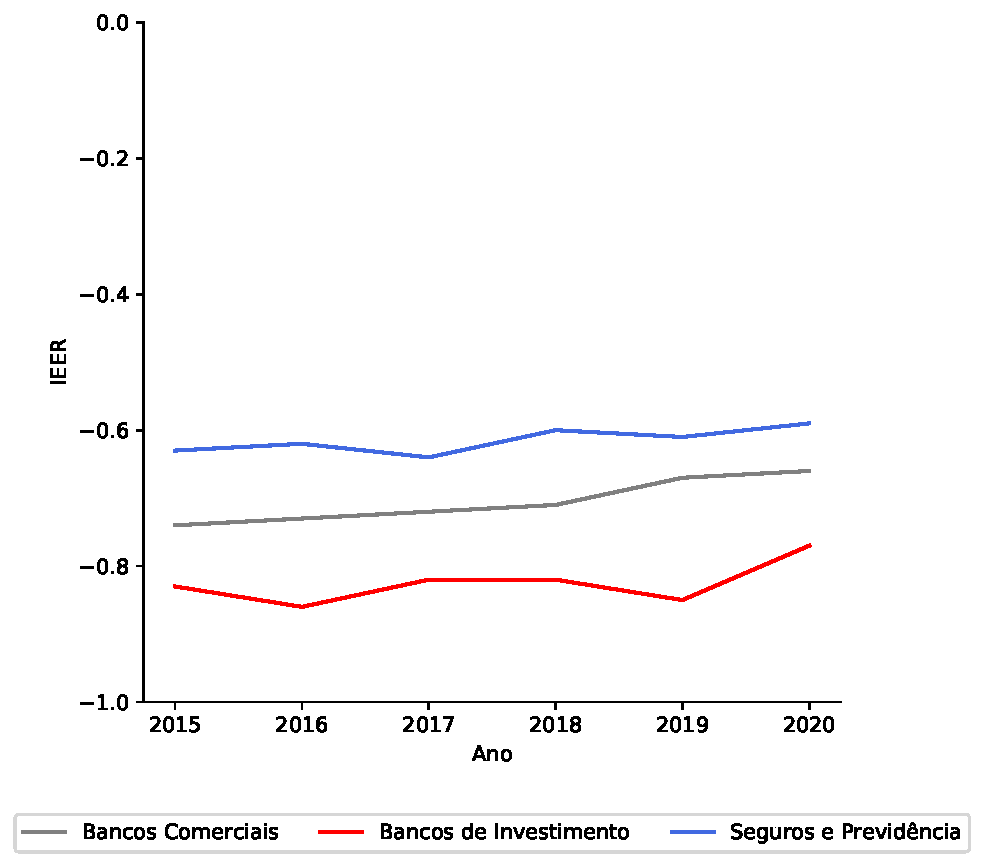
\includegraphics[height=12cm]{images/cnae_fin_ieer.pdf}
        \label{fig1}
    \end{figure} \label{ieer_ts}

\par Uma segundo fato que pode ser depreendido da observação das tabelas dessa subseção é a tendência dos Bancos Multiplos, com Carteira apresentarem os melhores indicadores de equidade racial, quando comparados com os demais grupos.

\clearpage

\section{Um exemplo} \label{als_study}

\par Nas seções anteriores deste trabalho, apresentaram-se o conceito do IEER e uma análise setorial que ajudou a indicar tendências gerais da equidade racial no mercado de trabalho paulista. Nesta breve seção, conclui-se esse relatório considerando o exemplo de uma empresa aderente ao pacto. A tabela 8 apresenta os dados de uma empresa fictícia com 2.270 colaboradores pertencente ao grupo de atividade de Bancos Comerciais.

\begin{table}[htb!]
\centering
\caption{Dados fictícios de um Banco Comercial }
\begin{tabular}{lccc}
\hline
Grupo ocupacional & Não-Liderança & Gerência & Diretoria \\ \hline
IEER              & -0.3          & -0.54    & -0.73     \\
Trabalhadores     & 2000          & 200      & 70        \\
Ensino Superior   & 800           & 180      & 70        \\
Ensino Médio      & 1200          & 20       & 0         \\
Negros            & 500           & 20       & 0         \\ \hline
\end{tabular}
\end{table} \label{example_company}

\par A partir dos dados apresentados na tabela 8 pode-se inferir que o $IEER^{I}$ da empresa é de -0,52. Se a empresa decide aderir ao Pacto e adotar 3 medidas associadas a políticas afirmativas, então seu IEER global será de -0,40. Para avançar mais no seu indicador global, a empresa precisa consultar seu Investimento Social de Referência que, no caso, será de aproximadamente 1.626.000, conforme fórmula apresentada na subseção \ref{levels3}.\footnote{O valor de \textit{p} de referência utilizado foi de 35\%.} Se a empresa decide aportar 40\% desse valor, então serão somados 0,08 pontos ao seu IEER. Dessa forma, o IEER final da empresa será de -0,32. 

% \section{Conclusão} \label{conclusion}

\clearpage

\appendix


\section{Padronização IEER} \label{standard_ieer}

\par Para chegar à versão padronizada são necessários mais alguns passos, em relação à equação \ref{eqv} apresentada no texto principal. Assim, usando propriedades da distribuição binomial, pode-se substituir $bn$ por $x$:

\begin{equation}
    \frac{n(b-p)}{\sqrt{n p \left(1 - p\right)}}
\end{equation}

\par Elevando ao quadrado e aplicando a raiz quadrada:

\begin{equation}
    \sqrt{\frac{n^{2}\left(b - p\right)^{2}}{n p \left(1 - p\right)}}    
\end{equation}


\begin{equation}
    \sqrt{\frac{n\left(b - p\right)^{2}}{p \left(1 - p\right)}}    
\end{equation}

\par Como $b$ é uma proporção, seu valor necessariamente varia de 0 a 1. Assim, é possível definir dois limites para $v$ como função de $b$. Se $b=0$, vale:

\begin{equation}
    \sqrt{\frac{np^{2}}{p \left(1 - p\right)}}    
\end{equation}

\begin{equation}
    \sqrt{\frac{np}{\left(1 - p\right)}}    
\end{equation}

\par Se $b=1$:

\begin{equation}
    \sqrt{\frac{n\left(1 - p\right)^{2}}{p \left(1 - p\right)}}    
\end{equation}

\begin{equation}
    \sqrt{\frac{n\left(1 - p\right)}{p}}
\end{equation}

\par Então, uma versão padronizada do índice pode ser construída dividindo-se $v$ por:

\begin{equation}
    \frac{\sqrt{n p^{1 - b} \left(1 - p\right)^{b}}}{\sqrt{p^{b} \left(1 - p\right)^{1 - b}}}
\end{equation}

\par Realizando a divisão:

\begin{equation}
    \psi = \frac{\frac{n(b-p)}{\sqrt{n p \left(1 - p\right)}}}{\frac{\sqrt{n p^{1 - b} \left(1 - p\right)^{b}}}{\sqrt{p^{b} \left(1 - p\right)^{1 - b}}}}
\end{equation}

\begin{equation}
    \psi = \frac{n(b-p)}{\sqrt{n p \left(1 - p\right)}} \cdot \frac{\sqrt{p^{b} \left(1 - p\right)^{1 - b}}}{\sqrt{n p^{1 - b} \left(1 - p\right)^{b}}}
\end{equation}


\begin{equation}
    \psi = \frac{n(b-p)}{\sqrt{n p \left(1 - p\right)}} \cdot \frac{1}{\sqrt{n p(1-p)}} \cdot \sqrt{\frac{p^{b}(1 - p)^{1 - b}}{p^{-b}(1 - p)^{b-1}}}
\end{equation}

\begin{equation}
    \psi = \frac{n(b-p)}{n p \left(1 - p\right)} \cdot \frac{p^{2b}}{(1-p)^{2(b+1)}}
\end{equation}

\begin{equation}
    \psi \frac{b-p}{(1-p)^{b}p^{1-b}}
\end{equation}

\par O \textit{IEER} é simplesmente um rearranjo da expressão acima:

\begin{equation}
    IEER = \frac{b-p}{p \left(\frac{1-p}{p}\right)^{b}}
\end{equation}

\clearpage

\printbibliography[title={Bibliografia}, nottype=misc]

\end{document}